\documentclass{article}
\usepackage[utf8]{inputenc}
\usepackage{hyperref}
\usepackage[letterpaper, portrait, margin=1in]{geometry}
\usepackage{enumitem}
\usepackage{amsmath}
\usepackage{booktabs}
\usepackage{graphicx}
\usepackage{amsmath}
\usepackage{hyperref}
\hypersetup{
colorlinks=true,
    linkcolor=black,
    filecolor=black,      
    urlcolor=blue,
    citecolor=black,
}
\usepackage{natbib}
\usepackage{titlesec}
\titleformat{\section}
{\normalfont\Large\bfseries}{\thesection}{1em}{}[{\titlerule[0.8pt]}]

\title{ECON7103HW5}
\author{Sedat Ors}
\date{20 February 2024}

\begin{document}

\maketitle

\section{Python}

\begin{enumerate}

\item The coefficient of mpg and constants are -22.2121 and 22482.7955, respectively. This means price will drop by 22.21 when mpg is increased 1 unit.

\item There may be several reasons for endogeneity. For example car brand can be important, or the weights of the drivers or passengers can be important, or usage of type of fuel can also be important. 

\item
\begin{itemize}
    \item a) See table \ref{tab:question3}, coloumn 1
    \item b) See table \ref{tab:question3}, coloumn 2
    \item c) See table \ref{tab:question3}, coloumn 3
    \begin{table}[ht]
  \centering
    \begin{tabular}{@{\extracolsep{5pt}}lccc}
\\[-1.8ex]\hline
\hline \\[-1.8ex]
& \multicolumn{3}{c}{\textit{Dependent variable:}} \
\cr \cline{3-4}
\\[-1.8ex] & (1) & (2) & (3) \\
\hline \\[-1.8ex]
 MPG & 150.43$^{}$ & 157.06$^{**}$ & 10165.74$^{}$ \\
  & (62.83) & (62.02) & (26559.83) \\
 Car type (Sedan) & -4676.39$^{}$ & -4732.67$^{***}$ & -90156.39$^{}$ \\
  & (576.35) & (573.29) & (226687.35) \\
 Constant & & 17441.23$^{***}$ & -264024.20$^{}$ \\
  & & (1751.12) & (746919.27) \\
\hline \\[-1.8ex]
 F-test for Stage 1 & 75.46 & 75.77 & 0.0 \\
 Observations & 1,000 & 1,000 & 1,000 \\
 $R^2$ & 0.19 & 0.20 & 0.19 \\
 Adjusted $R^2$ & 0.19 & 0.19 & 0.19 \\
 Residual Std. Error & 3491.04 & 3480.12 & 3491.04  \\
 F Statistic & 118.09$^{***}$  & 121.97$^{***}$  & 118.09$^{***}$  \\
\hline
\hline \\[-1.8ex]
\textit{Note:} & \multicolumn{3}{r}{$^{*}$p$<$0.1; $^{**}$p$<$0.05; $^{***}$p$<$0.01} \\
\end{tabular}
    \caption{2SLS results with 95\% confidence level}
    \label{tab:question3}
\end{table}
  

\item d) Exclusion in instrumental variable is  an assumption that a particular instrument used in the model is not directly related to the outcome variable, and is only related to the endogenous explanatory variables through the effect it has on the explanatory variables. The excluded instrument should influence price by mpg. These instruments seems not reasonable.

\item e) The results of mpg is very similar in model 1 and model 2, and they are significant. However in model 3, the F statistic is not significant. we can say that height can not be a good IV. 

\end{itemize}

\item The coefficient of IV GMM is 150.43 and the standart error is 63.051 as lower CI is 26.856 and upper CI is 274. in model 1 and 2 the standart errors are 62.83 and 62.02, respectively. So they seem similar but, the interval is a bit higher. Therefore, we should use robust standart error. 

\end{enumerate}

\section{Stata}
\begin{enumerate}
\item See Table \ref{tab:my_image}

\begin{table}[h]
    \centering
    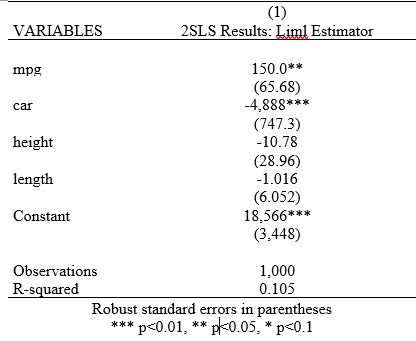
\includegraphics[width=0.5\textwidth]{table1.png}
    \caption{LIML Regression results}
    \label{tab:my_image}
\end{table}


\item The 5\% critical value is 37.418 and the F statistic is 94.05 in Table \ref{tab:my_image1}. Therefore, we can reject the H0 hypothesis that says the instrumental is weak.

\begin{table}[h]
    \centering
    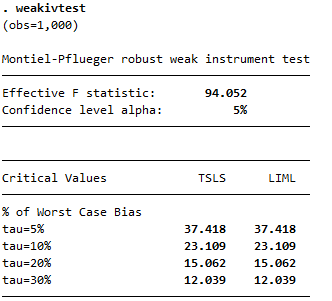
\includegraphics[width=0.5\textwidth]{table3 (2).png}
    \caption{Montiel-Pflueger results}
    \label{tab:my_image1}
\end{table}

\end{enumerate}

\end{document}
